\pdfoptionpdfminorversion=5
\documentclass[handout, 10pt, aspectratio=169, c ,hyperref={pdfpagelabels=false}]{beamer}
\usepackage{pgfpages}
\usepackage[ngerman]{babel}
\usepackage[utf8]{inputenc}
\usepackage{times}
\usepackage[T1]{fontenc}
\usepackage{amsmath}
\usepackage{graphicx}
\usepackage{hyperref}
\usepackage{xmpmulti}
\usepackage{multicol}
\usepackage{icomma}
\usepackage{booktabs}
\usepackage{array}
\usepackage{hyperref}
\usepackage{caption}
\usepackage{subcaption}

\newcolumntype{L}[1]{>{\raggedright\let\newline\\\arraybackslash\hspace{0pt}}m{#1}}
\newcolumntype{R}[1]{>{\raggedleft\let\newline\\\arraybackslash\hspace{0pt}}m{#1}}
\newcolumntype{C}[1]{>{\centering\let\newline\\\arraybackslash\hspace{0pt}}m{#1}}

\newcommand{\backgroundRef}{background \href{https://www.freepik.com/free-photo/beautiful-milky-way-night-sky_18667464.htm\#query=presentation\%20background\&position=1\&from_view=keyword}{image by rawpixel.com} on Freepik}

\mode<presentation>

\setbeamercolor{normal text}{fg=white}
\setbeamercolor{alerted text}{fg=red}
\setbeamercolor{example text}{fg=green}
\setbeamercolor{structure}{fg=white}

\setbeamercolor{block title}{use=structure,fg=structure.fg,bg=structure.fg!30}
\setbeamercolor{block title alerted}{use=alerted text,fg=alerted text.fg,bg=alerted text.fg!30}
\setbeamercolor{block title example}{use=example text,fg=example text.fg,bg=example text.fg!30}

\setbeamercolor{block body}{parent=normal text,use=block title,bg=block title.fg!10}
\setbeamercolor{block body alerted}{parent=normal text,use=block title alerted,bg=block title alerted.fg!10}
\setbeamercolor{block body example}{parent=normal text,use=block title example,bg=block title example.fg!10}

% Template
\defbeamertemplate*{headline}{default theme}{\vskip.5cm}
\defbeamertemplate*{footline}{default theme}{
    \hskip5pt
    \textcolor{white}{
        \bf \insertframenumber{} / \inserttotalframenumber \hspace*{.5cm} \backgroundRef{} \hspace*{9.75cm} \href{https://github.com/jaess105/Vortrag-Programmiersprachen}{GitHub} 
    }
    \vskip3.2pt
}
\setbeamertemplate{frametitle}{\color{white}\insertframetitle\par \vspace*{.5cm} \insertframesubtitle}
\setbeamertemplate{navigation symbols}{}
\mode<all>

\usebackgroundtemplate{
    
\includegraphics[width=\paperwidth]{../head/fig/gradient-dark-dynamic-lines-background/5570834}
}

% "hhuBlau" muss gesetzt sein damit es mit dem Template der HHU funktioniert.
% "backgroundNormal", "backgroundTitle" und "backgroundEmpty" auch.
\colorlet{hhuBlau}{white}


\newcommand{\backgroundNormal}{
    % \usebackgroundtemplate{
    % \includegraphics[width=\paperwidth]{head/fig/background_cd_2020}}
}
\newcommand{\backgroundTitle}{
    % \usebackgroundtemplate{
    % \includegraphics[width=\paperwidth]{head/fig/background_heine}}
}
\newcommand{\backgroundEmpty}{
    % \usebackgroundtemplate{
    % \includegraphics[width=\paperwidth]{head/fig/background_empty}}
}

\setlength{\leftmargini}{9pt}
\setbeamersize{text margin left=25pt,text margin right=25pt}
\setbeamertemplate{itemize/enumerate subbody end}{\vspace{.5\baselineskip}}
\setbeamertemplate{section in toc}[sections numbered]

\newenvironment<>{todoblock}{\setbeamercolor{block title}{fg=white,bg=orange}\setbeamercolor{block body}{bg=orange!10}\begin{block}#1{WORKING UNIT}}{\end{block}}
\newenvironment<>{exercise}[1]{\setbeamercolor{block title}{fg=white,bg=red}\setbeamercolor{block body}{bg=red!10}\setbeamercolor{itemize item}{fg=red}\begin{block}{Aufgabe (#1)}}{\end{block}}
\newenvironment<>{infoblock}[1]{\setbeamercolor{block title}{fg=white,bg=white}\setbeamercolor{block body}{bg=white!10}\setbeamercolor{itemize item}{fg=white}\begin{block}{#1}}{\end{block}}

\author{Jannik Esser}
\date{\today}
\usepackage{xcolor}
\usepackage{eurosym}

\definecolor{md-red}{HTML}{C62828}
\definecolor{md-purple}{HTML}{8E24AA}
\definecolor{md-indigo}{HTML}{3949AB}
\definecolor{md-cyan}{HTML}{00BCD4}
\definecolor{md-teal}{HTML}{00695C}
\definecolor{md-grass}{HTML}{689F38}
\definecolor{md-gray}{HTML}{616161}
\definecolor{md-gray-dark}{HTML}{494949}
\definecolor{md-orange}{HTML}{FF8F00}
\definecolor{md-yellow}{HTML}{FFD600}
\definecolor{md-green}{HTML}{388E3C}

\usepackage[most]{tcolorbox}
\newtcolorbox{terminalbox}{
    top=0pt,
    bottom=0pt,
    enhanced,
    attach boxed title to top,
    boxed title style={colback=md-gray-dark, colframe=md-gray-dark, arc=.25cm, top=0mm, bottom=0mm},
    fonttitle=\color{white}\bf,
    colframe=md-gray-dark,
    arc=.25cm,
    title={Bash \$\_\hfill \tikz\draw[md-green,fill=md-green] (0,0) circle (1ex); \hspace{.5mm} \tikz\draw[md-yellow,fill=md-yellow] (0,0) circle (1ex); \hspace{.5mm} \tikz\draw[md-red,fill=md-red] (0,0) circle (1ex);}
}
\newtcolorbox{javabox}[1]{
    top=0pt,
    bottom=0pt,
    enhanced,
    attach boxed title to top,
    boxed title style={colback=md-teal, colframe=md-teal, arc=.25cm, top=0mm, bottom=0mm},
    fonttitle=\color{white}\bf,
    colframe=md-teal,
    arc=.25cm,
    title={#1\hfill \tikz\draw[md-green,fill=md-green] (0,0) circle (1ex); \hspace{.5mm} \tikz\draw[md-yellow,fill=md-yellow] (0,0) circle (1ex); \hspace{.5mm} \tikz\draw[md-red,fill=md-red] (0,0) circle (1ex);}
}


\newtcbox{\inlinecode}{on line, boxrule=0pt, boxsep=0pt, top=2pt, left=2pt, bottom=2pt, right=2pt, colback=gray!25, colframe=white, fontupper={\ttfamily \footnotesize}}


\usepackage{listings}
\lstdefinestyle{java}{
  showspaces=false,
  showtabs=false,
  breaklines=true,
  showstringspaces=false,
  breakatwhitespace=true,
  commentstyle=\color{md-gray},
  keywordstyle=\color{md-indigo}\bf,
  keywordstyle = [2]{\color{md-purple}\bf},
  keywordstyle = [3]{\color{md-gray}\bf},
  morekeywords = [1]{public, private, static, if, else, for},
  morekeywords = [2]{class, void, int, boolean, char, byte, return, double, String},
  morekeywords = [3]{},
  morestring=**[d]{"},
  stringstyle=\color{md-grass},
  morecomment=[l]{//},
  morecomment=[l]{<-},
  commentstyle=\color{md-orange}\bf,
  basicstyle=\mdseries,
  literate=
    {á}{{\'a}}1 {é}{{\'e}}1 {í}{{\'i}}1 {ó}{{\'o}}1 {ú}{{\'u}}1
    {Á}{{\'A}}1 {É}{{\'E}}1 {Í}{{\'I}}1 {Ó}{{\'O}}1 {Ú}{{\'U}}1
    {à}{{\`a}}1 {è}{{\`e}}1 {ì}{{\`i}}1 {ò}{{\`o}}1 {ù}{{\`u}}1
    {À}{{\`A}}1 {È}{{\'E}}1 {Ì}{{\`I}}1 {Ò}{{\`O}}1 {Ù}{{\`U}}1
    {ä}{{\"a}}1 {ë}{{\"e}}1 {ï}{{\"i}}1 {ö}{{\"o}}1 {ü}{{\"u}}1
    {Ä}{{\"A}}1 {Ë}{{\"E}}1 {Ï}{{\"I}}1 {Ö}{{\"O}}1 {Ü}{{\"U}}1
    {â}{{\^a}}1 {ê}{{\^e}}1 {î}{{\^i}}1 {ô}{{\^o}}1 {û}{{\^u}}1
    {Â}{{\^A}}1 {Ê}{{\^E}}1 {Î}{{\^I}}1 {Ô}{{\^O}}1 {Û}{{\^U}}1
    {ã}{{\~a}}1 {ẽ}{{\~e}}1 {ĩ}{{\~i}}1 {õ}{{\~o}}1 {ũ}{{\~u}}1
    {Ã}{{\~A}}1 {Ẽ}{{\~E}}1 {Ĩ}{{\~I}}1 {Õ}{{\~O}}1 {Ũ}{{\~U}}1
    {œ}{{\oe}}1 {Œ}{{\OE}}1 {æ}{{\ae}}1 {Æ}{{\AE}}1 {ß}{{\ss}}1
    {ű}{{\H{u}}}1 {Ű}{{\H{U}}}1 {ő}{{\H{o}}}1 {Ő}{{\H{O}}}1
    {ç}{{\c c}}1 {Ç}{{\c C}}1 {ø}{{\o}}1 {å}{{\r a}}1 {Å}{{\r A}}1
    {€}{{\euro}}1 {£}{{\pounds}}1 {«}{{\guillemotleft}}1
    {»}{{\guillemotright}}1 {ñ}{{\~n}}1 {Ñ}{{\~N}}1 {¿}{{?`}}1 {¡}{{!`}}1 
}
\makeatletter % we need to use kernel commands

\newcommand{\WithImages}[1]{%
    \begin{columns}
        \begin{column}{.7\framewidth}
            #1
        \end{column}
        \begin{column}{.2\framewidth}
            \checknextarg}

            \newcommand{\checknextarg}{\@ifnextchar\stopimages{ \stopImageTaking }{ \slurpNextArg }}
            \newcommand{\slurpNextArg}[1]{ \includegraphics[width=2cm]{#1} \checknextarg}
            \newcommand{\stopImageTaking}[1]{ \end{column} \end{columns} }

\makeatother

\newcommand{\imgWithSource}[3]{
    \includegraphics[width=2cm]{#1} \\
    \tiny Source:\thinspace{\tiny #2} \\
    \hbox{\tiny Content:\thinspace{\tiny\itshape #3}}
}

\newcommand{\textWithImages}[2]{
    \begin{columns}
        \begin{column}{.7\framewidth}
            #1
        \end{column}
        \begin{column}{.2\framewidth}
            #2
        \end{column}
    \end{columns}
}

\newcommand{\newSectionPage}[2]{
    \backgroundEmpty

    \begin{frame}
        \vfill
        \centering
        \begin{beamercolorbox}[sep=8pt,center,shadow=true,rounded=true]{title}
            \usebeamerfont{title}#1\par%
        \end{beamercolorbox}
        \vfill

        \note{
            #2
        }
    \end{frame}

    \backgroundNormal
}




\title{Programmiersprachen}
\subtitle{Ein genereller Überblick, welche es gibt und wo sie verwendet werden.}


\begin{document}

% TITELFRAME BITTE NICHT ÄNDERN
\backgroundTitle
\begin{frame}
    \thispagestyle{empty}
    \begin{columns}
        \column{0.4\paperwidth}{\footnotesize\color{hhuBlau}\put(20,-200){\insertdate}}
        \column{0.6\paperwidth}
        \color{hhuBlau}
        \LARGE \inserttitle\\[\baselineskip]
        \large \insertauthor
    \end{columns}
\end{frame}
\backgroundNormal

\section{Einleitung}

\section{Einführung}

% Überlegung. Wenn Programmiersprachen aufgelistet werden und dann die Gebiete unter die sie fallen,
% dann verliert man den Überblick welche Programmiersprachen für welche Gebiete verwendet werden können.
% Wenn die Gebiete und dann die Programmiersprachen, die für sie infrage kommen aufgelistet werden, 
% dann wird der Fokus von den Programmiersprachen wegbewegt und eher zu den Gebieten hinbewegt.
% Proposal:
% 1. Eine Auflistung von allen gebieten und was ihre Rolle ist.
% 2. Facetten von Programmiersprachen Einführung (Paradigmen, Typsicherheit...)
% 3. Durchgehen der verschiedenen Programmiersprachen. Listen wofür sie sinnvoll sind.
% 4. Zusammenfassung der Gebiete und welche Programmiersprachen für sie relevant sind
%    als Abschluss mit schnellem durchgehen der Folien zum späteren Nachlesen bei Interesse.
%
% Notes:
% - Vortrag über Quantum Computing in den Cybersecurity Teil einbauen https://www.youtube.com/watch?v=D1RCj_g5amA&t=1970s
% - CLIPS als Beispiel einer hoch spezialisierten Sprache.
% - Mica Fragen, was für Programmiersprachen er so benutzt abgesehen von Python.

% INHALTSVERZEICHNIS (GGF. ENTFERNEN)
\begin{frame}{Inhalt}
    \thispagestyle{empty}
    \tableofcontents
\end{frame}

\section{Hintergrundwissen}

\input{_Gebietserklärung.tex}

\subsection{Unterschiede in Programmiersprachen}

\begin{frame}{Paradigmen}

\end{frame}

\begin{frame}{Typsicherheit}

\end{frame}

\begin{frame}{Statically vs. dynamically typed}

\end{frame}

\begin{frame}{Compiled vs. interpreted}

\end{frame}

\begin{frame}{Garbage collected vs. manuelle Speicherallokation}

\end{frame}

\section{Programmiersprachen}

\begin{frame}{HTML \& CSS}
    \begin{columns}
        \begin{column}{.5\framewidth}

        \end{column}
        \begin{column}{.4\framewidth}
            
\includegraphics[width=2cm]{resources/logos/CSS3_HTML5}
        \end{column}
    \end{columns}
\end{frame}
\begin{frame}{JavaScript und TypeScript}
    \begin{columns}
        \begin{column}{.5\framewidth}

        \end{column}
        \begin{column}{.4\framewidth}
            
\includegraphics[width=2cm]{resources/logos/js}
            
\includegraphics[width=2cm]{resources/logos/ts}
        \end{column}
    \end{columns}
\end{frame}
\begin{frame}{PHP}
    \begin{columns}
        \begin{column}{.5\framewidth}

        \end{column}
        \begin{column}{.4\framewidth}
            
\includegraphics[width=2cm]{resources/logos/php}
        \end{column}
    \end{columns}
\end{frame}
\begin{frame}{Ruby}
    \begin{columns}
        \begin{column}{.5\framewidth}

        \end{column}
        \begin{column}{.4\framewidth}
            
\includegraphics[width=2cm]{resources/logos/ruby}
        \end{column}
    \end{columns}
\end{frame}

\begin{frame}{Java und die JVM}
    \begin{columns}
        \begin{column}{.5\framewidth}
            Java, Kotlin, Clojure, Scala
        \end{column}
        \begin{column}{.4\framewidth}
            
\includegraphics[width=2cm]{resources/logos/java}
        \end{column}
    \end{columns}
\end{frame}

\begin{frame}{Kotlin}
    \begin{columns}
        \begin{column}{.5\framewidth}

        \end{column}
        \begin{column}{.4\framewidth}
            
\includegraphics[width=2cm]{resources/logos/kotlin}
        \end{column}
    \end{columns}
\end{frame}
\begin{frame}{Dart}
    \begin{columns}
        \begin{column}{.5\framewidth}

        \end{column}
        \begin{column}{.4\framewidth}
            
\includegraphics[width=2cm]{resources/logos/dart}
        \end{column}
    \end{columns}
\end{frame}
\begin{frame}{Golang}
    \begin{columns}
        \begin{column}{.5\framewidth}

        \end{column}
        \begin{column}{.4\framewidth}
            
\includegraphics[width=2cm]{resources/logos/go}
            % 
\includegraphics[width=2cm]{resources/logos/go-mascot.png}
        \end{column}
    \end{columns}
\end{frame}
\begin{frame}{C, C++ \& Rust}
    \begin{columns}
        \begin{column}{.5\framewidth}

        \end{column}
        \begin{column}{.4\framewidth}
            
\includegraphics[width=2cm]{resources/logos/c}
            
\includegraphics[width=2cm]{resources/logos/cpp}
            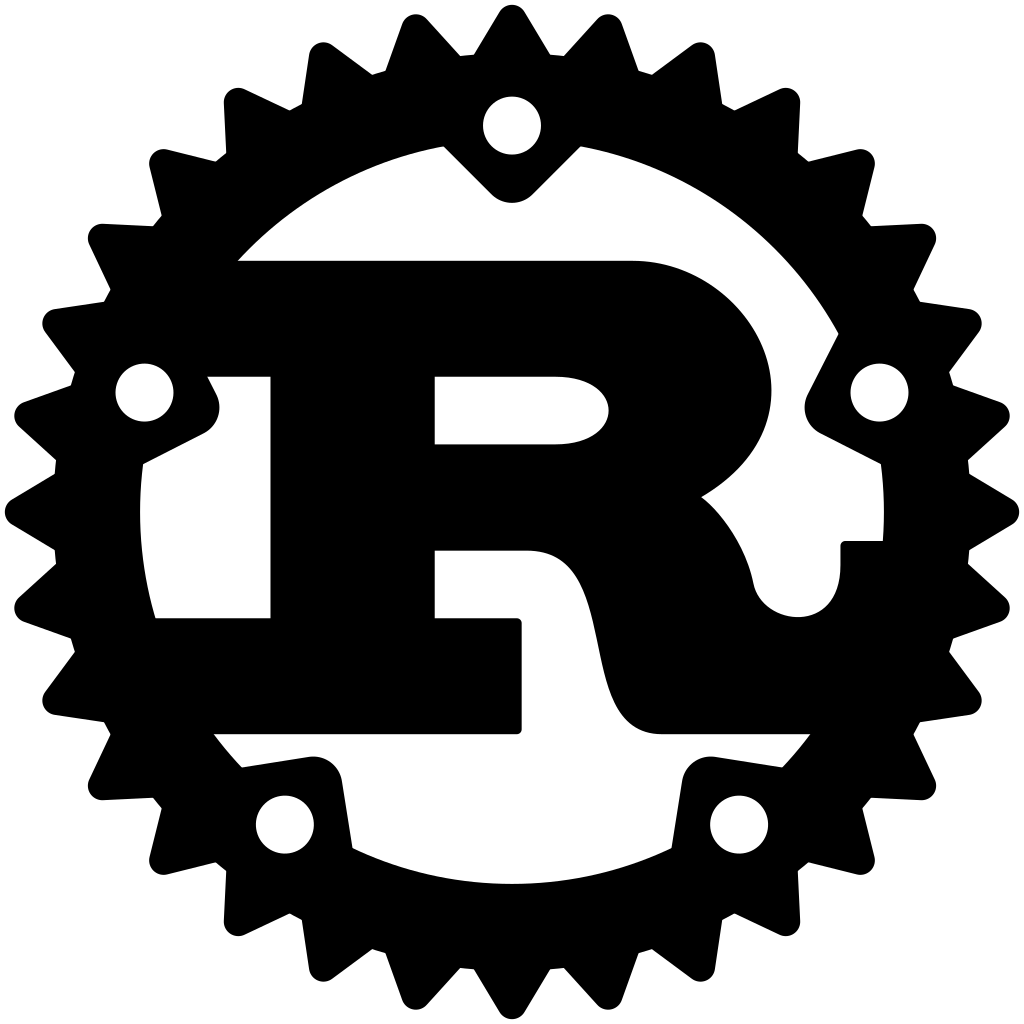
\includegraphics[width=2cm]{resources/logos/rust}
            
\includegraphics[width=2cm]{resources/logos/rust-mascot}
        \end{column}
    \end{columns}
\end{frame}

\begin{frame}{C\# und das .NET Framework}
    \begin{columns}
        \begin{column}{.5\framewidth}

        \end{column}
        \begin{column}{.4\framewidth}
            
\includegraphics[width=2cm]{resources/logos/csharp}
        \end{column}
    \end{columns}
\end{frame}

\begin{frame}{Python}
    \begin{columns}
        \begin{column}{.5\framewidth}

        \end{column}
        \begin{column}{.4\framewidth}
            
\includegraphics[width=2cm]{resources/logos/python}
        \end{column}
    \end{columns}
\end{frame}
\begin{frame}{Objective-C und Swift}
    \begin{columns}
        \begin{column}{.5\framewidth}

        \end{column}
        \begin{column}{.4\framewidth}
            
\includegraphics[width=2cm]{resources/logos/objective-c.png}
            
\includegraphics[width=2cm]{resources/logos/swift.png}
        \end{column}
    \end{columns}
\end{frame}
\begin{frame}{R \& Matlab}
    \begin{columns}
        \begin{column}{.5\framewidth}

        \end{column}
        \begin{column}{.4\framewidth}
            
\includegraphics[width=2cm]{resources/logos/r.png}
            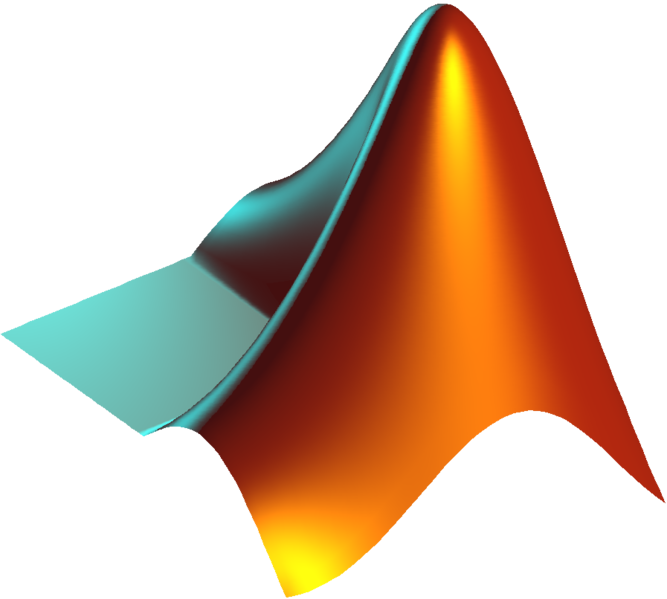
\includegraphics[width=2cm]{resources/logos/matlab.png}
        \end{column}
    \end{columns}
\end{frame}

\section{Zusammenfassung}

\begin{frame}{Zusammenfassung}
    Irgendwas richtig deepes.
\end{frame}


\begin{frame}[allowframebreaks]
    \frametitle{References}
    \bibliographystyle{unsrt}
    \bibliography{references} % Entries are in the references.bib file
\end{frame}




\end{document}